% Architecture diagram. Compile from this folder:
%   pdflatex -interaction=nonstopmode -halt-on-error -output-directory=../Figures fig_architecture.tex
% Include in main.tex:
%   
\includegraphics[width=\linewidth]{Figures/fig_architecture}
\documentclass[tikz,border=7pt]{standalone}
\usepackage[scaled=0.95]{helvet}
\renewcommand{\familydefault}{\sfdefault}
\usepackage{amsmath}
\usepackage{xcolor}
\usetikzlibrary{arrows.meta,positioning,fit,calc,backgrounds}

\definecolor{ink}{HTML}{1F2933}
\definecolor{muted}{HTML}{5B6776}
\definecolor{line}{HTML}{9AA7B5}
\definecolor{panel}{HTML}{F7F9FC}
\definecolor{paneldeep}{HTML}{E8EEF5}
\definecolor{accent}{HTML}{255E88}
\definecolor{train}{HTML}{EAF4EC}
\definecolor{lossfill}{HTML}{FFF4E3}

\begin{document}
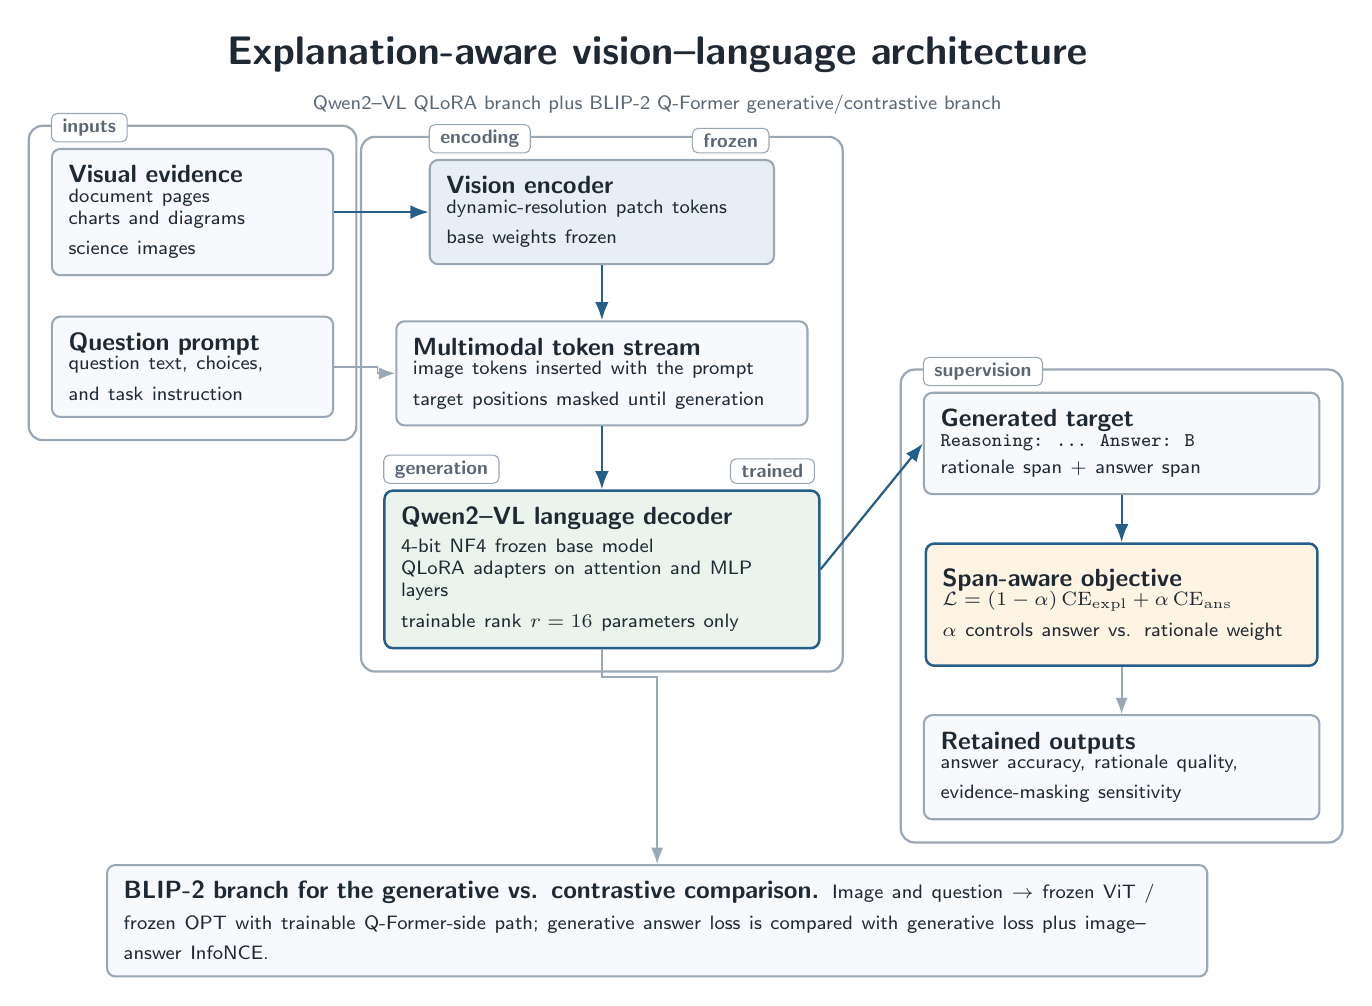
\begin{tikzpicture}[
  font=\sffamily\small,
  >=Latex,
  arrow/.style={->,line width=0.8pt,draw=accent},
  softarrow/.style={->,line width=0.65pt,draw=line},
  card/.style={draw=line,fill=panel,rounded corners=3pt,line width=0.75pt,
               inner sep=6pt,align=left,text=ink},
  frozen/.style={card,fill=paneldeep},
  trained/.style={card,fill=train,draw=accent,line width=0.9pt},
  loss/.style={card,fill=lossfill,draw=accent,line width=0.9pt},
  chip/.style={draw=line,rounded corners=2pt,fill=white,inner xsep=4pt,inner ysep=2pt,
               font=\scriptsize\bfseries,text=muted},
  title/.style={font=\sffamily\Large\bfseries,text=ink},
  subtitle/.style={font=\sffamily\scriptsize,text=muted}
]

\node[title] (title) at (7.8,9.35) {Explanation-aware vision--language architecture};
\node[subtitle,below=1pt of title] {Qwen2--VL QLoRA branch plus BLIP-2 Q-Former generative/contrastive branch};

% Inputs
\node[card,text width=3.15cm,minimum height=1.55cm] (image) at (1.9,7.35)
  {\textbf{Visual evidence}\\[-1pt]
   \scriptsize document pages\\ charts and diagrams\\ science images};
\node[card,text width=3.15cm,minimum height=1.25cm,below=5mm of image] (prompt)
  {\textbf{Question prompt}\\[-1pt]
   \scriptsize question text, choices,\\ and task instruction};

% Vision and token construction
\node[frozen,text width=3.95cm,minimum height=1.15cm,right=12mm of image] (vision)
  {\textbf{Vision encoder}\\[-1pt]
   \scriptsize dynamic-resolution patch tokens\\
   \scriptsize base weights frozen};
\node[card,text width=4.8cm,minimum height=1.15cm,below=7mm of vision] (stream)
  {\textbf{Multimodal token stream}\\[-1pt]
   \scriptsize image tokens inserted with the prompt\\
   \scriptsize target positions masked until generation};

% Decoder
\node[trained,text width=5.1cm,minimum height=2.0cm,below=8mm of stream] (decoder)
  {\textbf{Qwen2--VL language decoder}\\[2pt]
   \scriptsize 4-bit NF4 frozen base model\\
   \scriptsize QLoRA adapters on attention and MLP layers\\
   \scriptsize trainable rank $r=16$ parameters only};
\node[chip,anchor=south east] at ($(decoder.north east)+(-2pt,2pt)$) {trained};
\node[chip,anchor=south east] at ($(vision.north east)+(-2pt,2pt)$) {frozen};

% Target and supervision
\node[card,text width=4.6cm,minimum height=1.25cm,right=13mm of decoder,yshift=16mm] (target)
  {\textbf{Generated target}\\[-1pt]
   \scriptsize \texttt{Reasoning: ... Answer: B}\\[-1pt]
   \scriptsize rationale span + answer span};
\node[loss,text width=4.55cm,minimum height=1.55cm,below=6mm of target] (loss)
  {\textbf{Span-aware objective}\\[-1pt]
   \scriptsize $\mathcal{L}=(1-\alpha)\,\mathrm{CE}_{\mathrm{expl}}+\alpha\,\mathrm{CE}_{\mathrm{ans}}$\\
   \scriptsize $\alpha$ controls answer vs. rationale weight};
\node[card,text width=4.6cm,minimum height=1.1cm,below=6mm of loss] (eval)
  {\textbf{Retained outputs}\\[-1pt]
   \scriptsize answer accuracy, rationale quality,\\ evidence-masking sensitivity};

% BLIP-2 reference lane
\node[card,text width=13.55cm,minimum height=1.0cm] (blip) at (7.8,-1.65)
  {\textbf{BLIP-2 branch for the generative vs. contrastive comparison.}
   \scriptsize Image and question $\rightarrow$ frozen ViT / frozen OPT with trainable Q-Former-side path;
   generative answer loss is compared with generative loss plus image--answer InfoNCE.};

% Section labels
\node[chip,anchor=south west] at ($(image.north west)+(0,2pt)$) {inputs};
\node[chip,anchor=south west] at ($(vision.north west)+(0,2pt)$) {encoding};
\node[chip,anchor=south west] at ($(decoder.north west)+(0,2pt)$) {generation};
\node[chip,anchor=south west] at ($(target.north west)+(0,2pt)$) {supervision};

% Arrows
\draw[arrow] (image.east) -- (vision.west);
\draw[softarrow] (prompt.east) -- ++(0.55,0) |- (stream.west);
\draw[arrow] (vision.south) -- (stream.north);
\draw[arrow] (stream.south) -- (decoder.north);
\draw[arrow] (decoder.east) -- (target.west);
\draw[arrow] (target.south) -- (loss.north);
\draw[softarrow] (loss.south) -- (eval.north);
\draw[softarrow] (decoder.south) -- ++(0,-0.35) -| (blip.north);

% Light grouping panels
\begin{scope}[on background layer]
  \node[draw=line,fill=white,rounded corners=5pt,line width=0.8pt,
        fit=(image)(prompt),inner sep=8pt] {};
  \node[draw=line,fill=white,rounded corners=5pt,line width=0.8pt,
        fit=(vision)(stream)(decoder),inner sep=8pt] {};
  \node[draw=line,fill=white,rounded corners=5pt,line width=0.8pt,
        fit=(target)(loss)(eval),inner sep=8pt] {};
\end{scope}

\end{tikzpicture}
\end{document}
